\section{Einstieg}

\begin{frame}{Problemstellung}
	\begin{itemize}
		\item Punkte nach Dichtefunktion im Raum verteilen
		\item<2-> Mehrere existierende Verfahren
		\begin{itemize}
			\item Halton \small(\cite{wong_luk_heng-halton_points_sampling-1997})\normalsize
			\item Blue Noise \small(\cite{yan-blue_noise_sampling-2015})\normalsize
		\end{itemize}
		\item<3-> \textit{Erweiterung:} gleichmäßige Verteilung
		\begin{itemize}
			\item Golden Ratio Sequences + Halton/Blue Noise \small(\cite{schretter-golden_ratio_sequences-2012})\normalsize
			\item Fibonacci Grids \small(\cite{frisch_hanebeck-deterministic_gaussian_sampling-2021})\normalsize
		\end{itemize}
		\item<4->\textbf{Ziel 1:} effizientes Vorgehen 
		\item<5->\textbf{Ziel 2:} mehrdimensional anwendbar
		\item<6->\textbf{Ziel 3:} unabhängig von bestimmten Eigenschaften der Funktion einsetzbar
	\end{itemize}
\end{frame}

\begin{frame}{Ziel}
	\begin{figure}
		\begin{subfigure}{.45\textwidth}
			\centering
			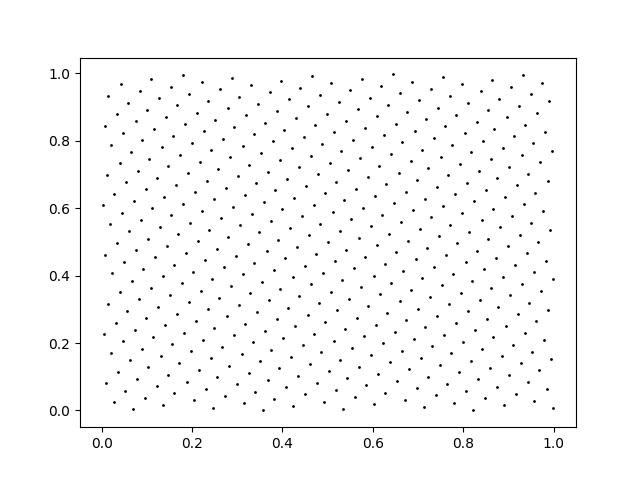
\includegraphics[width=\textwidth]{pdf_plots/grs_u500c.pdf}
		\end{subfigure}
		% \hfill
		% \begin{subfigure}{.15\textwidth}
		% 	\centering
		% 	
\includegraphics[width=.5\textwidth, angle=180]{Screenshots/img_71815.png}
		% \end{subfigure}
		% \hfill
		\begin{subfigure}{.45\textwidth}
			\centering
			\includegraphics[width=\textwidth]{pdf_plots/idf2_log-log_iu500c-GRS.pdf}
		\end{subfigure}
		\caption{\small\cite{schretter-golden_ratio_sequences-2012}\normalsize}
	\end{figure}
\end{frame}